\documentclass[11pt,a4paper]{article}

\usepackage[utf8]{inputenc}
\usepackage[T1]{fontenc}
\usepackage{geometry}
\usepackage{graphicx}
\usepackage{hyperref}
\usepackage{xcolor}
\usepackage{listings}
\usepackage{float}

\geometry{margin=2.5cm}

\hypersetup{
    colorlinks=true,
    linkcolor=black,
    urlcolor=blue
}

\lstset{
    basicstyle=\ttfamily\small,
    frame=single,
    breaklines=true,
    columns=fullflexible
}

\title{Projet de Recherche Opérationnelle\\
\large Flot maximum et flot maximum de coût minimum}
\author{Bence Di Placido}
\date{\today}

\begin{document}

\begin{titlepage}
    \centering
    \vspace*{2cm}
    
\includegraphics[width=0.4\textwidth]{resources/LogoUCA.png}\\[1cm]
    {\Huge \bfseries Projet de Recherche Opérationnelle\\[0.5cm] \Large Flot maximum et flot maximum de coût minimum avec détection de cycles négatif}\\[2cm]
    {\Large Bence Di Placido}\\[1cm]
    {\large \today}
    \vfill
\end{titlepage}
\tableofcontents
\newpage
\section{Introduction}

Le but de ce projet est de manipuler des graphes de flot en Java. On part d'un
graphe orienté où chaque arc possède une capacité, et éventuellement un coût.
Le programme doit lire ce graphe depuis un fichier texte, calculer une solution,
puis produire une visualisation du graphe avant et après le calcul en fournissant le flot maximum, la min cut et le coût si demandé.

Deux problèmes sont traités. Le premier est le problème classique du flot
maximum : on cherche à envoyer le plus de flot possible depuis une source
\texttt{s} vers un puits \texttt{t}, sans dépasser les capacités des arcs. Le
deuxième est une variante plus complète : parmi les flots maximums possibles,
on veut trouver un flot dont le coût total est minimum.

Le projet a donc été organisé autour de trois étapes assez simples :
\begin{enumerate}
    \item construire le graphe à partir d'un fichier d'entrée ;
    \item appliquer l'algorithme choisi ;
    \item exporter le résultat en DOT/PDF pour vérifier visuellement le flot,
    les coûts et la coupe minimale.
\end{enumerate}

J'ai essayé de garder une structure lisible plutôt que de tout mettre dans une
seule classe. Même si le projet reste de taille raisonnable, séparer les modèles,
les constructeurs et les algorithmes permet de mieux comprendre où chaque
responsabilité se trouve.

\section{Format d'entrée et sortie du programme}

Le fichier d'entrée contient d'abord une ligne avec le nombre de noeuds, le
nombre d'arcs, l'indice de la source et l'indice du puits :

\begin{lstlisting}
nombre_noeuds nombre_arcs source puits
\end{lstlisting}

Ensuite, chaque ligne décrit un arc :

\begin{lstlisting}
source destination capacite cout
\end{lstlisting}

Par exemple, le graphe utilisé dans les tests contient 6 noeuds, 10 arcs, la
source d'indice 5 et le puits d'indice 4. Dans le programme, la source est
renommée \texttt{s} et le puits \texttt{t}, ce qui rend la lecture des graphes
plus claire.

Après l'exécution, le programme génère deux versions du graphe :
\begin{itemize}
    \item une version initiale, avant le calcul ;
    \item une version résultat, avec les flots calculés, le flot maximum, le
    coût total et les arcs de la coupe minimale mis en évidence.
Il est également possible de génerer les graphe résiduels de toutes les étapes qui ont permis a résoudre le flot.
\end{itemize}

\section{Structures de données}

\subsection{Représentation des noeuds}

Les noeuds sont représentés par une classe abstraite \texttt{Node}. Elle contient
un identifiant, un nom et une liste d'arcs sortants. Trois classes spécialisées
héritent ensuite de \texttt{Node} :
\begin{itemize}
    \item \texttt{StartNode} pour la source ;
    \item \texttt{MiddleNode} pour les noeuds intermédiaires ;
    \item \texttt{EndNode} pour le puits.
\end{itemize}

Ce choix n'est pas obligatoire pour résoudre le problème : on aurait pu utiliser
une seule classe \texttt{Node} avec un attribut indiquant le type du noeud. J'ai
préféré les classes séparées car elles rendent le modèle plus explicite. Quand
on lit le code, on voit directement quel noeud joue le rôle de source et quel
noeud joue le rôle de puits.

\subsection{Représentation des arcs}

Chaque arc est représenté par la classe \texttt{Arc}. Elle stocke :
\begin{itemize}
    \item la source et la destination ;
    \item la capacité restante ;
    \item la capacité initiale ;
    \item le flot actuellement envoyé ;
    \item le coût de passage sur l'arc.
\end{itemize}

La capacité initiale est gardée séparément de la capacité courante. Ce choix est
utile car les algorithmes modifient les capacités dans le graphe résiduel, alors
que l'affichage final doit encore connaître la capacité de départ. Sans cette
information, il serait plus difficile d'afficher des labels du type
\texttt{flot/capacité}.

\subsection{Représentation du graphe}

La classe \texttt{Graph} regroupe la source, le puits, les noeuds intermédiaires
et plusieurs informations de résultat : le flot maximum, le coût total et la
coupe minimale. Le graphe est représenté principalement avec des listes
d'adjacence : chaque noeud possède sa liste d'arcs sortants.

J'ai choisi les listes d'adjacence plutôt qu'une matrice de capacités. Une
matrice est pratique pour accéder très vite à une capacité entre deux noeuds,
mais elle oblige à réserver une case pour chaque paire de noeuds, même quand il
n'y a pas d'arc. Ici les graphes sont naturellement orientés et peuvent être
plutôt creux, donc une liste d'adjacence est plus simple et plus économique en
mémoire. Elle correspond aussi bien aux parcours utilisés par BFS et
Bellman-Ford, qui inspectent les arcs sortants d'un noeud.

\subsection{Graphe résiduel}

Le graphe résiduel est construit par \texttt{ResidualGraphBuilder}. Pour chaque
arc original, le constructeur crée deux arcs :
\begin{itemize}
    \item un arc direct, avec la capacité disponible ;
    \item un arc inverse, avec une capacité initialement nulle et un coût opposé.
\end{itemize}

L'arc inverse est essentiel. Il permet à l'algorithme de revenir sur une décision
ancienne si un meilleur chemin est trouvé ensuite. Dans le cas du coût minimum,
son coût négatif représente le fait qu'annuler du flot annule aussi le coût
payé auparavant.

Le graphe garde aussi plusieurs \texttt{Map} :
\begin{itemize}
    \item une correspondance entre arc résiduel et arc original ;
    \item une indication pour savoir si un arc résiduel est inverse ou non ;
    \item une correspondance entre chaque arc résiduel et son arc opposé.
\end{itemize}

Ces tables ajoutent un peu de complexité, mais elles évitent de modifier
directement le graphe original pendant la recherche. Le résultat final reste
ainsi plus propre : le graphe original porte les flots finaux, tandis que le
graphe résiduel sert au calcul.

Une autre possibilité aurait été de stocker directement une référence vers l'arc
original dans chaque arc résiduel. J'ai préféré utiliser des \texttt{Map}, car
cela garde la classe \texttt{Arc} assez générale : un arc ne sait pas s'il vient
du graphe original ou du graphe résiduel. Les correspondances sont gérées par le
constructeur du graphe résiduel, ce qui centralise cette logique au même endroit.

\section{Construction du graphe}

La classe \texttt{GraphBuilder} lit le fichier texte ligne par ligne. Les lignes
vides et les commentaires sont ignorés, ce qui rend les fichiers d'entrée plus
faciles à écrire et à modifier.

La première ligne permet de créer tous les noeuds. Ensuite, chaque ligne d'arc
est vérifiée puis convertie en objet \texttt{Arc}. Le programme refuse les
capacités négatives, les arcs vers des noeuds inexistants et les fichiers dont
le nombre d'arcs ne correspond pas à l'en-tête.

J'ai choisi de valider les erreurs dès la lecture plutôt que de laisser
l'algorithme tomber plus tard sur un graphe incohérent. 

\section{Algorithme de flot maximum}

Pour le flot maximum sans coût, le projet utilise Ford-Fulkerson dans sa version
Edmonds-Karp. Le principe est le suivant :
\begin{enumerate}
    \item construire le graphe résiduel ;
    \item chercher un chemin augmentant de \texttt{s} vers \texttt{t} ;
    \item envoyer sur ce chemin le maximum possible, c'est-à-dire le minimum des
    capacités restantes du chemin ;
    \item mettre à jour les arcs directs et inverses du graphe résiduel ;
    \item recommencer tant qu'il existe un chemin augmentant.
\end{enumerate}

La différence avec un Ford-Fulkerson très général est que le chemin augmentant
est trouvé avec un BFS. Cela correspond à Edmonds-Karp. Ce choix est plus stable
qu'une recherche arbitraire en profondeur, car le BFS prend toujours un chemin
avec un nombre minimal d'arcs. En pratique, cela évite certains comportements où
Ford-Fulkerson peut faire beaucoup de petites augmentations peu efficaces.

Après la fin de l'algorithme, les noeuds encore atteignables depuis la source
dans le graphe résiduel sont calculés. Les arcs originaux qui partent d'un noeud
atteignable vers un noeud non atteignable forment une coupe minimale. Le
programme les garde pour les afficher en rouge dans le fichier DOT.

\section{Algorithme de flot maximum de coût minimum}

Pour la version avec coûts, l'idée reste proche : on augmente le flot dans le
graphe résiduel. La différence est le choix du chemin. Au lieu de prendre le
plus court chemin en nombre d'arcs, on prend le chemin de coût total minimal.

Pour trouver ce chemin, le projet utilise Bellman-Ford. Ce choix est important
parce que le graphe résiduel contient des arcs inverses avec des coûts négatifs.
Dijkstra aurait été plus rapide dans le cas de coûts tous positifs, mais il ne
fonctionne pas directement avec des coûts négatifs. Bellman-Ford est donc plus
adapté ici, même s'il est moins rapide.

À chaque itération :
\begin{enumerate}
    \item Bellman-Ford cherche un chemin de coût minimal entre \texttt{s} et
    \texttt{t} ;
    \item on calcule la capacité limitante du chemin ;
    \item on augmente le flot de cette quantité ;
    \item on ajoute au coût total le coût du chemin multiplié par la quantité de
    flot envoyée.
\end{enumerate}

Le programme vérifie aussi la présence d'un cycle de coût négatif atteignable.
Ce contrôle est nécessaire : avec un tel cycle, on pourrait diminuer le coût
indéfiniment dans le graphe résiduel, ce qui rendrait la notion de coût minimum
problématique.

\section{Visualisation}

L'export est fait avec Graphviz. La classe \texttt{DotPdfExporter} écrit d'abord
un fichier DOT, puis appelle la commande \texttt{dot} pour produire un PDF. Les
arcs affichent le flot et la capacité en bleu, puis le coût en rouge. La source
est colorée en vert et le puits en bleu.

Cette visualisation est utile pour vérifier rapidement que le résultat a du sens.
Par exemple, sur le graphe fourni, les tests indiquent un flot maximum de 15.
Avec l'algorithme de coût minimum, le coût total attendu est 149.


\begin{figure}[H]
    \centering
    
\includegraphics[width=0.85\textwidth]{resources/results/graph.pdf}
    \caption{Graphe obtenu après le calcul sur l'exemple fourni.}
\end{figure}


\section{Exemple de résolution en coût minimum}

Pour illustrer le fonctionnement de l'algorithme de flot maximum de coût
minimum, on peut regarder le graphe fourni dans les ressources. Au départ, aucun
flot n'a encore été envoyé. Les arcs sont seulement définis par leur capacité et
leur coût. Dans les figures, le label bleu correspond à
\texttt{flot/capacité}, et le nombre rouge correspond au coût de l'arc.

\begin{figure}[H]
    \centering
    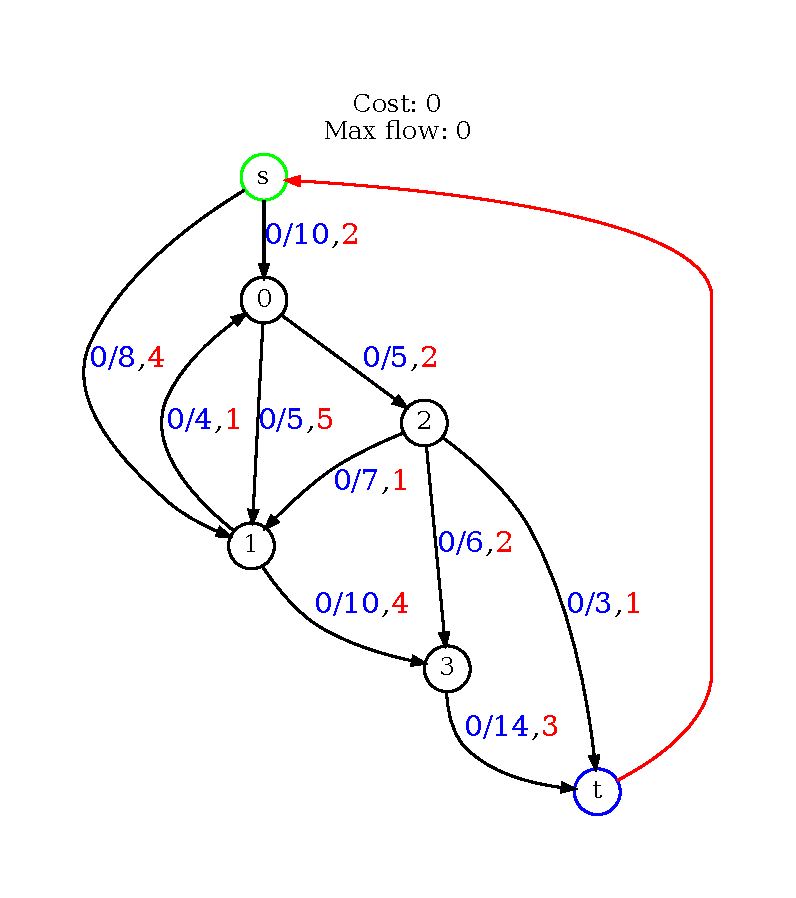
\includegraphics[width=0.5\textwidth]{resources/initials/graph.pdf}
    \caption{Graphe initial avant le calcul : toutes les valeurs de flot sont à 0.}
\end{figure}


Sur ce graphe initial, il faut trouver la solution avec le flot max qui coûte le moins cher. C'est
pour cela que l'algorithme ne prend pas simplement le premier chemin disponible :
à chaque étape, il cherche un chemin augmentant de coût minimal dans le graphe
résiduel.

\IfFileExists{resources/results/graph.pdf}{
\begin{figure}[H]
    \centering
    
\includegraphics[width=0.5\textwidth]{resources/results/graph.pdf}
    \caption{Graphe après résolution avec l'algorithme min-cost max-flow.}
\end{figure}
}{}

Le résultat obtenu est un flot maximum de 15 pour un coût total de 149. On voit
que les deux arcs qui sortent de la source sont utilisés : \texttt{s -> 0}
transporte 7 unités sur 10 possibles, et \texttt{s -> 1} transporte 8 unités sur
8. L'arc \texttt{s -> 1} est donc saturé.

Du côté du puits, le flot arrive par deux arcs : \texttt{2 -> t} transporte 3
unités sur 3, et \texttt{3 -> t} transporte 12 unités sur 14. Le total entrant
dans \texttt{t} est donc bien $3 + 12 = 15$, ce qui correspond au flot maximum
affiché.

Les arcs en rouge plus épais représentent la coupe minimale trouvée après le calcul du flot max. Ici,
on retrouve notamment \texttt{0 -> 2} et \texttt{1 -> 3}, qui sont saturés dans
la solution. Cela signifie qu'une fois ces passages pleins, il n'existe plus de
chemin résiduel permettant d'envoyer davantage de flot de \texttt{s} vers
\texttt{t}. Le programme ne se contente donc pas de donner une valeur numérique :
il permet aussi de voir quels arcs limitent le réseau.

Le coût total de 149 vient de la somme des flots envoyés sur chaque arc,
multipliés par leurs coûts. Par exemple, envoyer du flot sur un arc de coût 1
est préférable à capacité égale, mais l'algorithme doit aussi respecter les
capacités et parfois utiliser des arcs plus chers pour atteindre le flot maximum.
C'est exactement l'intérêt du min-cost max-flow : garder le débit maximal, tout
en choisissant la combinaison de chemins la moins coûteuse possible.

\section{Tests}

Des tests JUnit sont présents pour vérifier les deux algorithmes. Pour
Ford-Fulkerson, le test vérifie que le flot maximum du graphe donné en exemple vaut 15 et que l'algorithme
peut être relancé deux fois sur le même graphe sans conserver un état incorrect.

Pour le flot de coût minimum, le test vérifie que le flot maximum vaut aussi 15
et que le coût total vaut 149 pour le graphe donné en exemple. Un autre test construit un petit graphe avec un
cycle de coût négatif atteignable et vérifie que l'algorithme le refuse.

Ces tests ne prouvent pas que le programme est parfait, mais ils couvrent les
cas principaux du projet : calcul du flot, calcul du coût et détection d'une situation problématique.

\section{Conclusion}

Pour conclure, ce projet montre surtout que les algorithmes de flot ne servent pas seulement à
résoudre des graphes abstraits. Edmonds-Karp permet de trouver la quantité
maximale que l'on peut faire passer d'une source vers un puits, par exemple dans
un réseau de transport, de routes, de données ou de production. La version
min-cost max-flow ajoute une idée importante : on garde le meilleur débit
possible, mais en cherchant en plus à réduire le coût total.

En modélisant des problèmes de tous les jours sous forme de graphe, on peut donc 
obtenir des réponses assez concrètes : combien peut-on envoyer au maximum, quels
passages bloquent le réseau, ou quelle organisation donne le même résultat pour
un coût plus faible. C'est ce qui rend ces algorithmes intéressants. Une fois le
problème bien traduit en source, puits, capacités et coûts, le calcul permet de
faire apparaître des solutions qui ne sont pas toujours évidentes à trouver.

De plus, ce projet m'a permis de mieu comprendre le fonctionnement des algorithmes de
 maximisation de flots notament a l'aide des graphes résiduels pour chaque étapes de la résolutin ainsi que le théroeme de min cut / max flow.



\newpage

\section{Résolution des exemples donner}

\subsection{Exemple 1 (txt donné sur discord)}
\subsubsection{Flot max}
\begin{figure}[H]
    \centering
    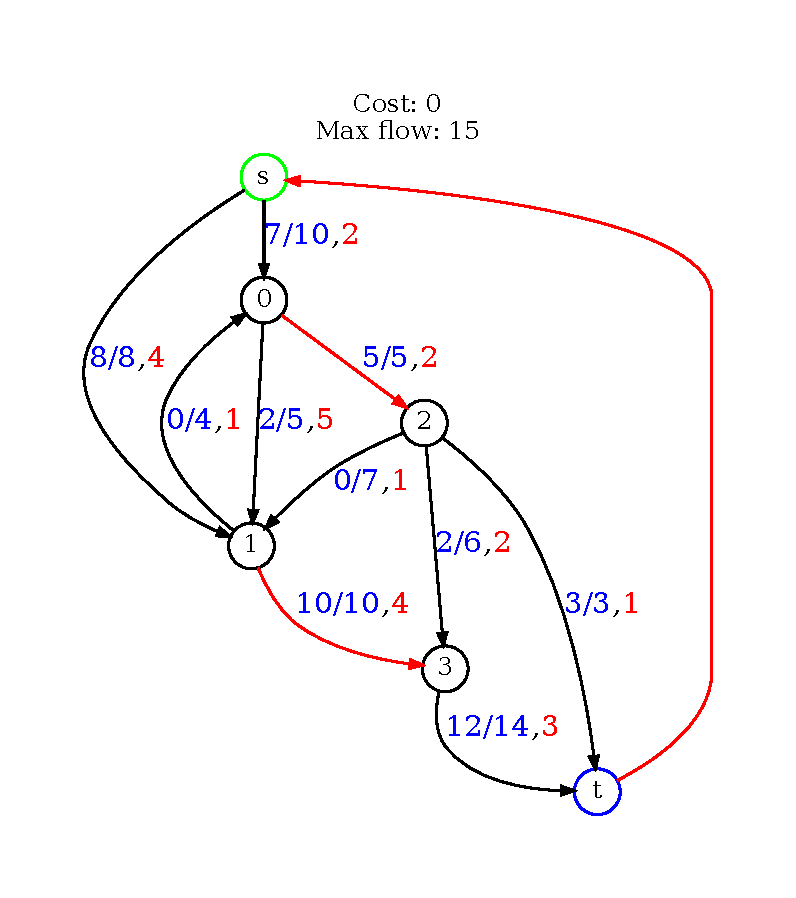
\includegraphics[width=0.6\textwidth]{resources/results/exemple.pdf}
    \caption{Graphe obtenu après le calcul du flot max.}
\end{figure}

On obtient un flot de 15 avec la coupe minimal qui contient les arcs saturés (0->2, 1->3)

\subsubsection{Flot max min cost (txt donné sur discord)}
\begin{figure}[H]
    \centering
    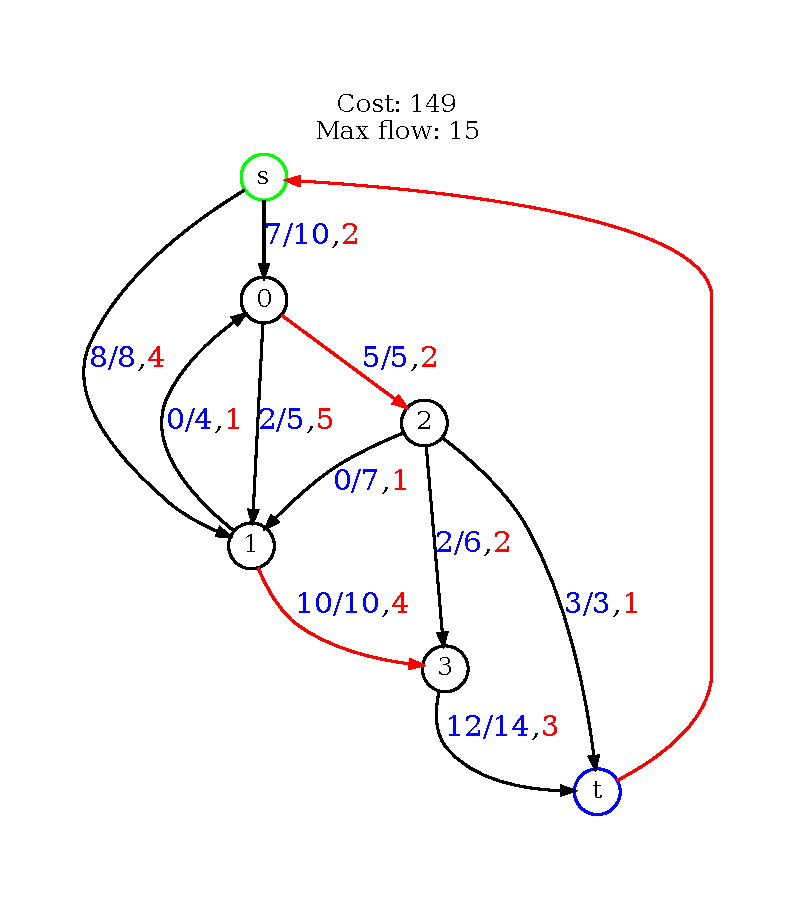
\includegraphics[width=0.6\textwidth]{resources/results/exemple_with_cost.pdf}
    \caption{Graphe obtenu après le calcul du min cost flot max.}
\end{figure}

On obtient un flot de 15 avec un coût de 149 et la coupe minimal qui contient toujours les arcs saturés (0->2, 1->3)

\subsection{Exercice 1 (fichier word)}
\begin{figure}[H]
    \centering
    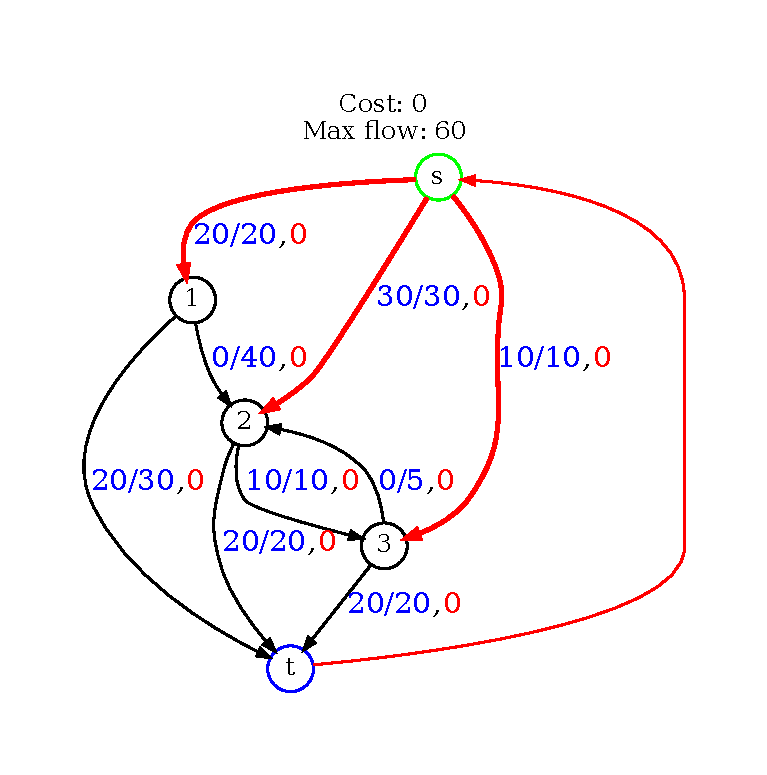
\includegraphics[width=0.6\textwidth]{resources/results/exo1_max_flow.pdf}
    \caption{Graphe obtenu après le calcul du flot max.}
\end{figure}

On obtient un flot de 60 avec la coupe minimal qui contient les arcs saturés (S->1, S->2, S->3)

\subsection{Exercice 2 (fichier word)}

\begin{enumerate}
    \item Sans capacité des tâches, on obtient un flot de 10 avec un coût de 370, les arcs de la min cut sont les arcs sortant de la source.
    \item Avec une capacité de 2 par tâches, on obtient un flot de 10 avec un coût de 404, les arcs de la min cut sont les arcs sortant de la source.
    \item Avec chaque tâche prise au moin une fois, on obtient un flot de 10 avec un coût de 413.
\end{enumerate}


\subsection{Exercice 3 (fichier word)}
\subsubsection{Flot max min cost dans (s,t)}
\begin{figure}[H]
    \centering
    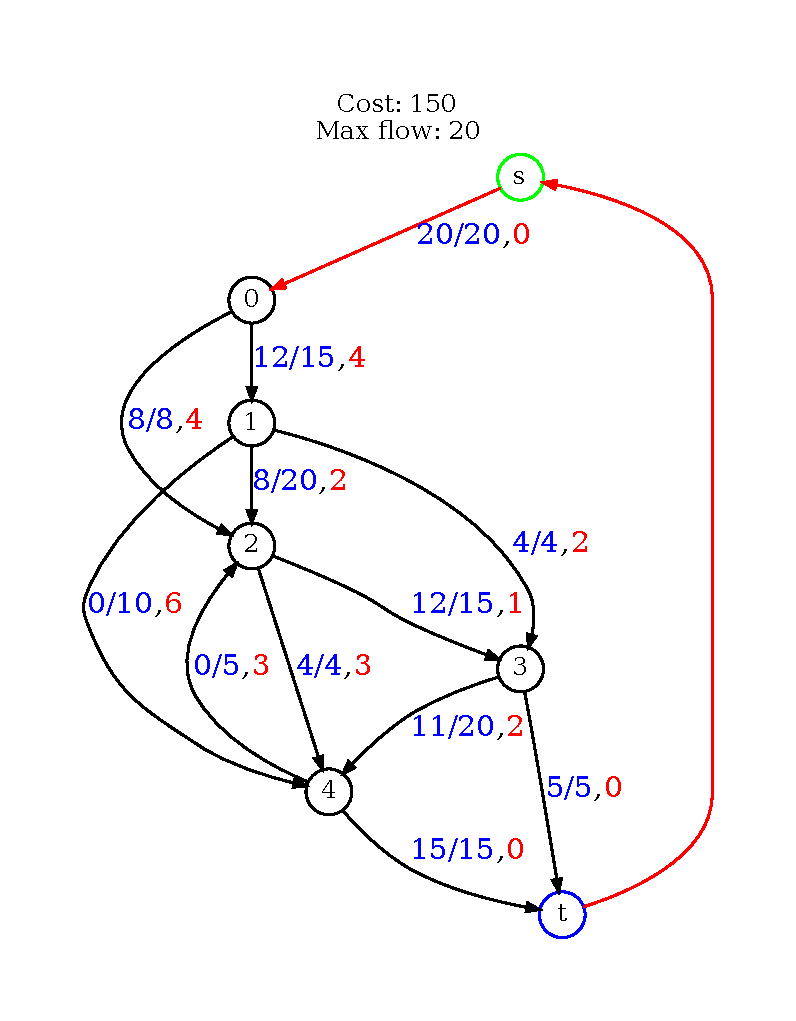
\includegraphics[width=0.6\textwidth]{resources/results/exo3_min_cost1.pdf}
    \caption{Graphe obtenu après le calcul du flot max min cost de (s,t).}
\end{figure}
On obtient un flot de 20 avec un coût de 150 et  la coupe minimal qui contient les arcs saturés (S->0)

\subsubsection{Flot max min cost dans (0,4)}
\begin{figure}[H]
    \centering
    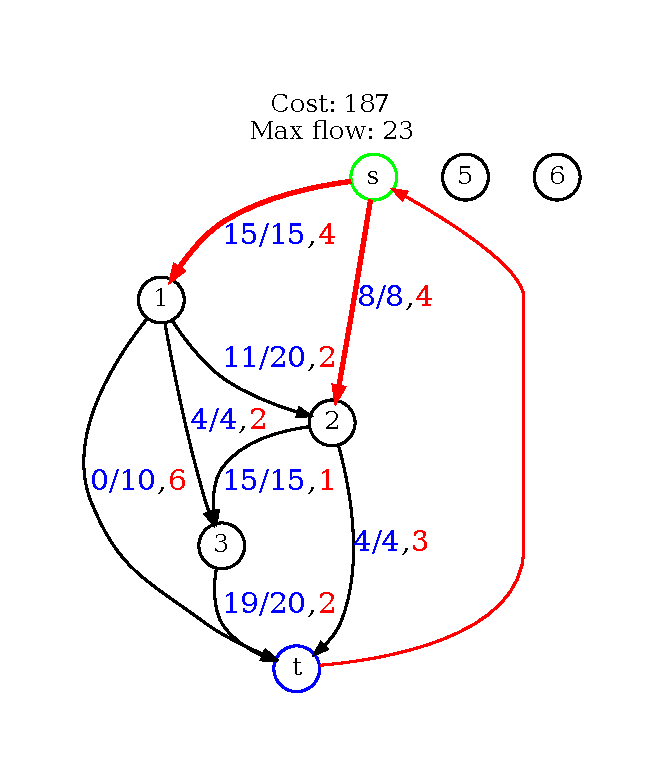
\includegraphics[width=0.6\textwidth]{resources/results/exo3_min_cost04.pdf}
    \caption{Graphe obtenu après le calcul du flot max min cost de (0,4).}
\end{figure}
On obtient un flot de 23 avec un coût de 187 et  la coupe minimal qui contient les arcs saturés (s->1, s->2) (s est 0)


\subsubsection{Most vital arc de (s,t) et (0,4)}
L'arc le plus vitale de (s,t) et l'arc s->0 car sans lui le flot est a 0. 
L'arc le plus vitale de (0,4) et l'arc 0->1 (s->1) car c'est le plus grand arc de la coupe min, on aura donc un flot max de 8 après suppression de l'arc. (Théoreme flot max coupe min)
\end{document}
